%!TEX root = ../master_thesis.tex

\chapter{Constructing quantitative fault trees}
\label{chap:quantitive_fault_tree}

Based on the qualitative fault tree structure, we would like to quantify the failure probabilities of the basic events to calculate the probability of the TOP event. The actual TOP event probability itself may not be useful in assessing the dependability of a system. But it is possible to evaluate how changes to basic event probabilities affect the probability of the TOP event.

We base our investigation in this section on the fault tree from previous \nref{subsec:fault_tree_construction}, specifically shown in \autoref{fig:fault_tree_threaded_comments}.

To calculate the probability of the TOP event, we use the transformation rules as described earlier in \nref{subsec:theory_faulttree}, resulting in the following equation:

% \autoref{eq:quant_bool} shows the fault tree as a boolean logic equation:
%
% \begin{multline} \label{eq:quant_bool}
%    Top Event = \\
%       \shoveleft{( \operatorname{mysql} \vee \operatorname{authenticator} ) \quad \vee} \\
%       \shoveleft{\operatorname{memcached} \quad \vee} \\
%       \shoveleft{\operatorname{soundcloud} \quad \vee} \\
%       \shoveleft{\operatorname{threaded-comments}}
% \end{multline}

% \autoref{eq:quant_prob} shows the boolean logic equation from previous \autoref{eq:quant_bool} tranformed to an equation for calculating the top event probability.

{\scriptsize
\begin{multline} \label{eq:quant_prob}
  P(TOP Event) = \\
     \shoveleft{P(mysql) + P(authenticator) - P(mysql) * P(authenticator) +} \\
     \shoveleft{P(memcached) -} \\
     \shoveleft{(P(mysql) + P(authenticator) - P(mysql) * P(authenticator)) * P(memcached) +} \\
     \shoveleft{P(soundcloud) - }\\
     \shoveleft{(P(memcached) - (P(mysql) + P(authenticator) - P(mysql) * P(authenticator))} \\
     * P(memcached)) * P(soundcloud) + \\
     \shoveleft{P(threaded\mbox{-}comments) -} \\
     \shoveleft{(P(soundcloud) - (P(memcached) - (P(mysql) + P(authenticator) - P(mysql) * P(authenticator))} \\
     * P(memcached)) * P(soundcloud))) * P(threaded\mbox{-}comments)
\end{multline}
}

\clearpage

To solve the equation probabilities for all basic events are needed. Rausand et al~\cite{SysReliabilityTheory} (section 4.3.5) introduce three categories for approaches for handling probabilistic analyses of software failure. All of these assume a fault tree that includes software, hardware and other events.
\begin{tenumerate}
  \item \textbf{Assume the probability of software failure is zero} This approach assumes that software never fails. It therefore limits the probabilistic analysis to the other components. We use this approach for software components that the deployed method may not derive probabilities for, therefore we set these probabilities to 0.
  \item \textbf{Assume the probability of software failure is one} This approach assumes that software always fails. It is therefore very pessimistic, since even though we may assume that software will eventually fail, usually it is more dependable than that. We do not use this approach in our works.
  \item \textbf{Separate the analysis of the software} This approach proposes to use separate analysis methods for software and other components. The methods we propose here may be seen in the context of this category.
\end{tenumerate}

For assessing the basic event probabilities we investigated the following methods:
\begin{tenumerate}
  \item Source code metrics
  \begin{tenumerate}
    \item Lines of code
    \item Code churn
  \end{tenumerate}
  \item Operational availability
  \begin{tenumerate}
    \item External heartbeat measurements
    \item Production traffic measurements
  \end{tenumerate}
\end{tenumerate}

We executed each of these methods in the context of our case study. Please note that a quantitative analysis of the methods was out of scope for this work. We executed the methods to show their feasibility. We do however evaluate each method qualitatively.

\section{Via source code metrics}
\label{sec:source_code}

Source code metrics provide insights about the state of a software by analyzing source code and its meta data. In this section we describe two methods for deriving failure probabilities from source code metrics. For each method we explain how we executed it in our case study and discuss its results.

\subsection{Lines of code}
\label{subsec:loc}

The \emph{lines of code} (short: \emph{LOC}) of an application are all text lines that contribute to the codebase of it. Earlier in \nref{sec:software_environment_terminology} we assumed that each application has exactly one codebase and that we are able to map the application identifier to its codebase. In our case study this assumption is true for internal applications, but not for external applications. Thus we manually linked the external application identifiers to the appropriate codebases.

We manually acquired the codebases for each application in the fault tree. We then counted the lines of code for each codebase. Our measurement of LOC took all lines of text in the codebase into consideration. This included tests, deployment and build scripts, example code, documentation and comments. We did not take shared library code into consideration, except if they were included in the codebase (e.g. since they have been copied in).

The internal applications \emph{soundcloud}, \emph{threaded-comments} and \emph{authenticator} were measured with their versions from 28 April 2014. The external applications \emph{mysql} and \emph{memcached} were measured with the version numbers that were deployed in the case study on 28 April 2014. The results can be seen in \autoref{tab:loc}.

To use the lines of code in the fault tree, we have to transform them to failure probabilities. We do this based on the assumption that per 1000 lines of code (short: \emph{KLOC}), there are a number of bugs present in the code. McConnell et al \cite{McConnellSteve} surveyed papers comparing \emph{number of defects per KLOC}. The values range from 0.1 defects to 50 defects per KLOC. We optimistically chose the lower bound \emph{0.1 defects per KLOC} as ratio to estimate the number of defects in a codebase. We now have to transform these to failure probabilities, in order to use them in the fault tree. We do so by assuming that the higher number of defects has a failure probability of 0.1. We may then normalize the other defect numbers accordingly. Table \ref{tab:loc} shows the results of this method.

\begin{table}
  \label{tab:loc}
  \caption{Lines of code calculation in the case study with accompanying failure probabilities.}
  \begin{tabular}{ |l|l|l|l| }
    \hline
    Application & Lines of code & Estimated number of defects & Failure probability \\
    \hline
    soundcloud & 635436 & 63,5436 & 0,007402703 \\
    threaded-comments & 1163 & 0,1163 & 0,000013549 \\
    authenticator & 6747 & 0,6747 & 0,000078601 \\
    mysql & 8583837 & 858,3837 & 0,1 \\
    memcached & 28354 & 2,8354 & 0,000330318 \\
    \hline
  \end{tabular}
\end{table}

Given the resulting failure probabilities, we may now use these as basic event failure probabilities in earlier \autoref{eq:quant_prob} to calculate the TOP event probability. The resulting TOP event probability is \textbf{0,10704}.

\subsubsection{Discussion}

Both the functions for calculating defects per line as well as transforming defects to failure probabilities have been chosen by us as ``good guesses'', since these were not in the focus of this work. We believe that more work is needed in choosing appropriate functions and values.

Given the \emph{lines of code} numbers from table \ref{tab:loc}, we can see there is a large variance in the size of codebases in our case study. For example the \emph{mysql} codebase is more than 7000 times larger than the \emph{threaded-comments} codebase. The failure probabilities from this method are proportional to the lines of code. Therefore the calculated TOP event probability is highly influenced from the big codebases but does not respect smaller codebase well.

We calculated the \emph{lines of code} by summing up all text lines in a codebase. An opportunity for future work would be to investigate, in how much these numbers change, if only the code that is immediately used for running processes is taken into consideration.

\subsection{Relative code churn}
\label{subsec:relative_code_churn}

\emph{Code churn} is a measure based on summarizing the added and changed lines of code in a codebase for a period of time. In this subsection we will explain, how we used relative code churn to calculate the failure probability of an application.

In our case study, all internal applications' codebases were tracked in Git~\cite{ProGit}. Therefore we were able to use the approach by Kraaijeveld \cite{KaidencePost} for measuring code churn: For a git branch, gather all parent commits for the defined time period. For each commit, summarize the number of added lines. Summarize these numbers over all commits. The resulting number is the absolute code churn.

As shown by Nagappan et al \cite{Nagappan2005} relative code churn may be used as a predictor of defects in source code. Therefore, we normalize the absolute code churn by the lines of code at the time of the start of the measured period (as explained in~\cite{Nagappan2005} as measure \emph{M1}).

In our case study, relative code churn for own applications is relevant to the behavior of the deployed architecture, since deploys happen often (often within hours of the code changes being present in the codebase). We may therefore assume that the codebase's state matches the code that is deployed.

Table \ref{tab:app_churn} shows the results from calculating relative code churn over three time periods of one week, as well as over a time period of four months.

\begin{table}[!h]
  \caption{Relative code churn in the case study calculated over several time periods.}
  \label{tab:app_churn}
  \begin{tabular}{ |l|l|l|l| }
    \hline
    Application & Beginning LOC & Absolute churn & Relative churn \\
    \hline
    25 March 2014 - 31 March 2014 \\
    authenticator & 6981 & 42 & 0,006016 \\
    soundcloud & 635434 & 2478 & 0,003900 \\
    threaded-comments & 1163 & 1 & 0,000860 \\
    \hline
    01 April 2014 - 06 April 2014 \\
    authenticator & 6839 & 32 & 0,004679 \\
    soundcloud & 635571 & 326 & 0,000513 \\
    threaded-comments & 1163 & 4 & 0,003439 \\
    \hline
    18 April 2014 - 24 April 2014 \\
    authenticator & 6875 & 762 & 0,110836 \\
    soundcloud & 635165 & 893 & 0,001406 \\
    threaded-comments & 1163 & 0 & 0  \\
    \hline
    01 January 2014 - 30 April 2014 \\
    authenticator & 6322 & 3805 & 0,601866 \\
    soundcloud & 518904 & 33643 & 0,064835 \\
    threaded-comments & 1163 & 40 & 0,029235 \\
    \hline
  \end{tabular}
\end{table}

Assuming that relative code churn is a predictor for defect rates, we may also assume that it predicts the failure rates of the applications. Thus we use the relative code churn as basic event failure rates in earlier \autoref{eq:quant_prob} to calculate the TOP event probability. Table~\ref{tab:app_churn_fail} shows the results for the different time periods.

\begin{table}[!h]
  \centering
  \caption{Relative code churn in the case study: TOP event failure probabilities after the fault tree for several time periods.}
  \label{tab:app_churn_fail}
  \begin{tabular}{ |l|l| }
    \hline
    Application & Top event failure probability\\
    \hline
    25 March 2014 - 31 March 2014 & 0,010774 \\
    01 April 2014 - 06 April 2014 & 0,008610 \\
    18 April 2014 - 24 April 2014 & 0,112209 \\
    01 January 2014 - 30 April 2014 & 0,638560 \\
    \hline
  \end{tabular}
\end{table}

\subsubsection{Discussion}

We calculated the code churn for internal applications only, but did not take the external applications \emph{memcached} and \emph{mysql} into consideration. We based this decision on the fact that the deploys of both applications in our case study were not upgraded with new versions in the time of our investigation. Therefore their code churn would not influence the deployed architecture.

We base our assumptions about mapping relative code churn to defect probabilities on Nagappan et al \cite{Nagappan2005}. They investigated code churn on differences between software releases. We did our measurements in a continuous deployment environment without explicit releases. Instead of differences between releases we used arbitrary time periods to bound the code changes to include in the investigation. We did not investigate, how this change might alter the results. Future work should investigate the significance of relative code churn towards defect rates in a continuous deployment environment.

In our calculation of absolute code churn, we took into consideration all text in the codebase, regardless if it contributes to the running application. We did not evaluate how non-application text like tests, examples or documentation influence the results.

For calculating absolute churn, we did not take deleted code into consideration. This is due to the fact that in Git a modified line of code is expressed as an added and a deleted line, thus counting deleted lines would weight modified lines double and over-emphasize them against newly added lines. Furthermore we (similarly to \cite{KaidencePost}) assume that deleted code is a low-relevance churn operation.

We use relative code churn directly as failure probability. We may assume that the longer the time period for the measurement, the higher the code churn will be. This is visible in our results in \autoref{tab:app_churn}, where the relative churn numbers for weeks are magnitudes lower than the churn numbers over months. Relative code churn may then also exceed 1, when more lines have been added/changed than lines of codes existed at the begin of the time period. In that case, relative code churn could not be used anymore as failure probability directly, but would have to be normalized.

The code churn of a single application is highly influenced by the specifics of the development process used with regards to how changes to the codebase manifest themselves in the version control system. In our case study, all applications follow the same development process, loosely based on the model as outlined in \cite{GitFlow}. There, different branches (code versions) are used for developing a feature. Once the development on a feature is completed, its changes are reviewed and then merged into a central branch (example names are \emph{trunk}, \emph{stable} or \emph{master}). This branch is the one that is used while deploying. We also used that central branch for calculating code churn. Future work should investigate, to which extent other development processes influence the relative code churn and therefore the failure probabilities.

\section{Via historical availability data}
\label{sec:historical_availability}

To calculate the TOP event probability in a fault tree, we need to assign failure probabilities to the basic events. In this section we describe two methods for deriving basic event failure probabilities from historical availability data.

\subsection{Theory}
\label{subsec:historical_availability_theory}

Given that an application is deployed, we may measure the deploy's availability at runtime, which over a time period will provide us with the historical availability.

To acquire that data, we used two methods:
\begin{tenumerate}
  \item External heartbeat measurements
  \item Production traffic measurements
\end{tenumerate}

In both measurements, we derived a time series for each deploy in the production environment. Each time step in the series holds the information if the deploy was either \emph{up} or \emph{down} in that time period.

Figure \ref{fig:availability_timeseries} shows an example of such a time series. As we can see, there were two time periods where the application was successively \emph{down} (Minute 5 and minutes 9 to 10) as well as three time periods where the application was successively \emph{up} (Minutes 1 to 4, minutes 6 to 8 and minutes 11 to 12). The duration of each \emph{up} time period may also be called the \emph{time to failure}, thus the duration it took from getting to an initial \emph{up} state to the next \emph{down} state. Furthermore we may then calculate the average time it takes until failure, also called the \emph{mean time to failure} or \emph{MTTF}. Equation \ref{eq:mttf} shows how to calculate that from a time series. The execution for this with the example time series is visible in equation \ref{eq:mttf_example}.

\begin{figure}[ht]
  \centering
  
\includegraphics[width=0.7\columnwidth] {images/availability_timeseries.pdf}
  \caption{Historical availability: Example of time series for a time period of 12 minutes with \emph{1} representing ``up'' and \emph{0} representing ``down'' for the respective time step}
  \label{fig:availability_timeseries}
\end{figure}

\begin{equation} \label{eq:mttf}
  MTTF = \frac{\operatorname{Number\:of\:"up"\:steps}}{\operatorname{Number\:of\:sequences\:with\:coherent\:"up"\:states}}
\end{equation}

\begin{equation} \label{eq:mttf_example}
  MTTF_{example} = \frac{9}{3} = 3
\end{equation}

We assume that during the time of our measurement the system has reached steady-state, meaning that if we would execute the measurements over the same length but at different points in time, we would get the same MTTF value.

The software systems we investigate are by definition repairable. For example after a failure occurred a software system may continue to work as expected afterwards due to self-repair mechanisms or, if the cause of failure is a crash, by being restarted and therefore repaired externally. We work under the assumption here that these system repairs are perfect, thus that after a repair the system is ``as good as new''.

Given these assumptions, we may calculate the failure rate with equation \ref{eq:failurerate}:
\begin{equation} \label{eq:failurerate}
  \lambda = \frac{1}{\operatorname{MTTF}}
\end{equation}

As distribution for failure probability we assume an exponential distribution. Therefore the system is said to be ``without memory'': the probability of failure at any point in time is the same, regardless of the time that passed already. We may calculate the failure probability with equation \ref{eq:failureprob}:
\begin{equation} \label{eq:failureprob}
  Pr(t) = 1 - e^{- \lambda * t}
\end{equation}

The variable \emph{t} denotes the ``mission time''. Given a specific mission time \emph{t}, the probability \emph{Pr(t)} denotes the probability that the system has failed at or before that time. Intuitively we see that the longer the mission time is, the higher the probability that the system has failed will be.

Next we will describe the two methods we used for measuring the availability of systems. We executed both methods over the same period of seven days. We did not measure the applications \emph{memcached} and \emph{mysql} because no existing measuring mechanisms provided reasonable indicators for their availability.

\subsection{External heartbeat measurements}
\label{subsec:heartbeat_measurement}

To measure the availability of an application, we did regular requests to the deployed service instances of it. We will explain the method in detail next, then show our results from executing the method in our case study and end the section by discussing our findings.

\subsubsection{Measurement method}

To execute the measurements, we created our own measurement application (called \emph{measurer}). It ran on one machine within the internal network, being able to do network requests to all deployed service instances. We measured three applications: \emph{soundcloud}, \emph{authenticator} and \emph{threaded-comments}. Each application had one production deploy with many service instances. The instances were found via the Glimpse service discovery (as explained earlier in~\nref{subsubsec:glimpse}). All services used the HTTP~\cite{rfc2616} protocol. For the measurement we chose one HTTP resource for each application. \emph{Measurer} then requested that resource on all service instances of the deploy. Each HTTP request may either return an HTTP response with an HTTP status code, or may be a timeout if it has not returned after a certain period of time (in our case 30 seconds). For all resources we expected HTTP status code 200, if the call was successful. Thus, when a response with HTTP status code 200 was received, we defined that instance to be \emph{up}. If the HTTP status code was equal to or bigger than 500, or a timeout occurred, we define the instance to be \emph{down} for that period of time\footnote{During the investigations we did not receive any other HTTP status codes like 201 or 301, thus we were not concerned with them here.}.

To alleviate load and limit impact of the measurements on the running system, we only requested 10 instances of each deploy at a time, but requested all instances of each deploy eventually within one measurement step. In \autoref{fig:heartbeat_duration} are the total durations for querying all instances of an application in each measurement runs. For \emph{authenticator} and \emph{threaded-comments}, these always finished quickly. For \emph{soundcloud} these show some spikes, resulting from some requests timing out at the 30 second mark we set as timeout interval.

\begin{figure}[ht]
  \fbox{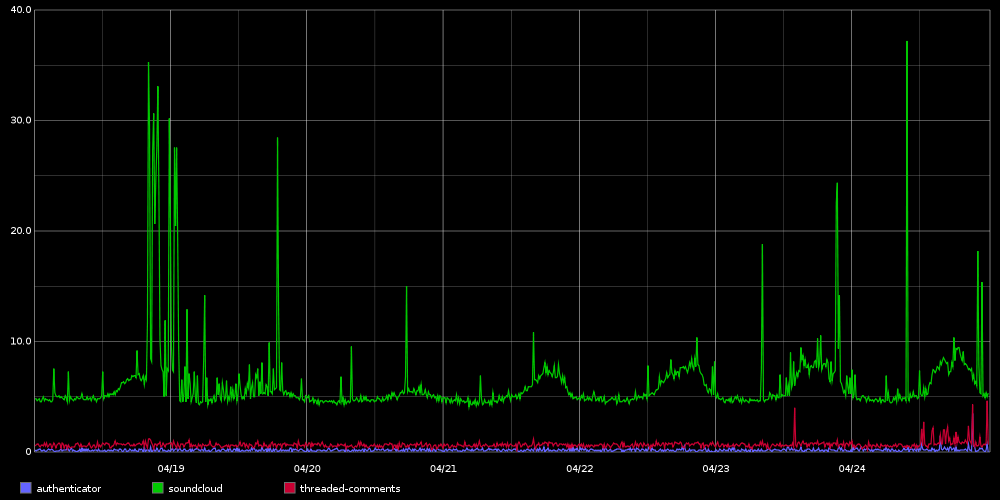
\includegraphics[width=\columnwidth] {images/availability/apr18/durations.png}}
  \caption{Heartbeat measurement: Duration of each measurement step for each application}
  \label{fig:heartbeat_duration}
\end{figure}

One measurement happened every minute. The measurements were executed continuously for seven days between April 18 2014 and April 24 2014 inclusively. The results were stored in a \emph{Graphite} server~\cite{graphite}, which allowed for extracting the raw time series data for further analysis but also generated the plotted visual graphs shown in this section.

\subsubsection{Results}

The results of our measurements can be seen in \autoref{fig:heartbeat_soundcloud}, \autoref{fig:heartbeat_auth} and \autoref{fig:heartbeat_tr}~\footnote{Due to the large time period represented in the plotted graphs, values are smoothed.}. Each figure holds the measurements for one application, with the responses of all instances summarized for each time period, with a plotted graph per status code. If an instance returned HTTP status code 200, we interpret that as ``\emph{instance is up}''. If an instance returned a status code in the 5XX range or the request timed out, we interpret that as ``\emph{instance is down}''. Next we will comment on each figure.

\begin{tdescription}
  \item[\autoref{fig:heartbeat_soundcloud} soundcloud] Around April 18 2014 3:00 there is an increase in \emph{200} status codes that is due to a provisioning of more instances. Around April 23 2014 14:00 there are some spikes in \emph{500/timeout}, which peak at about 30 instances.
  \item[\autoref{fig:heartbeat_auth} authenticator] Around April 22 2014 11:30 there is an increase in up and down instances. This increase is due to the experimental deployment of a development branch on one instance. The development branch was tested with different configurations against live traffic, some of which configurations did not deliver correct functionality. At April 24 2014 12:00 onwards there are occasional spikes in \emph{500/timeouts}. These peak at 2 instances and at maximum last 3 minutes.
  \item[\autoref{fig:heartbeat_tr} threaded-comments] At April 23 10:00 there is a spike of \emph{500/timeouts} that lasts for 14 minutes and peaks at 23 instances.
\end{tdescription}

\begin{figure}[ht]
  \fbox{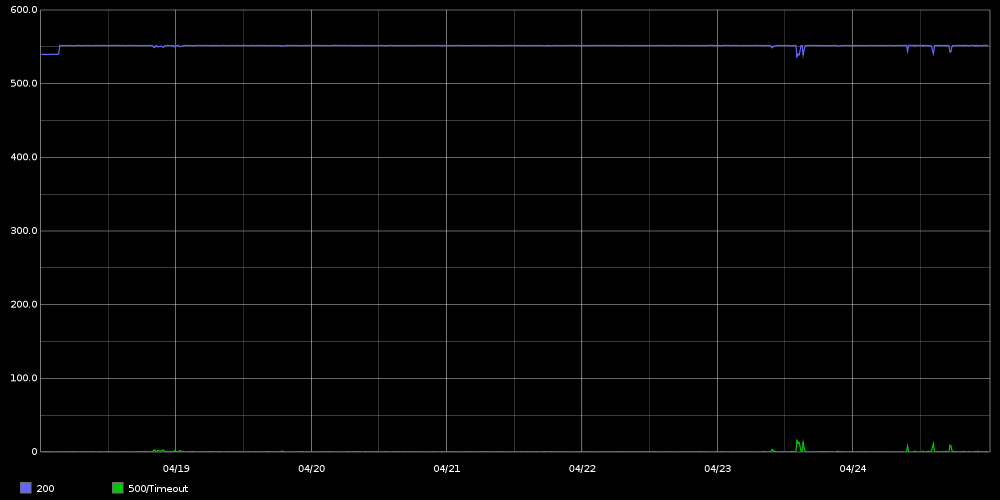
\includegraphics[width=\columnwidth] {images/availability/apr18/soundcloud_measurer_small.png}}
  \caption{Heartbeat measurement: Summarized HTTP request status codes for each measurement step for application \emph{soundcloud}}
  \label{fig:heartbeat_soundcloud}
\end{figure}

\begin{figure}[ht]
  \fbox{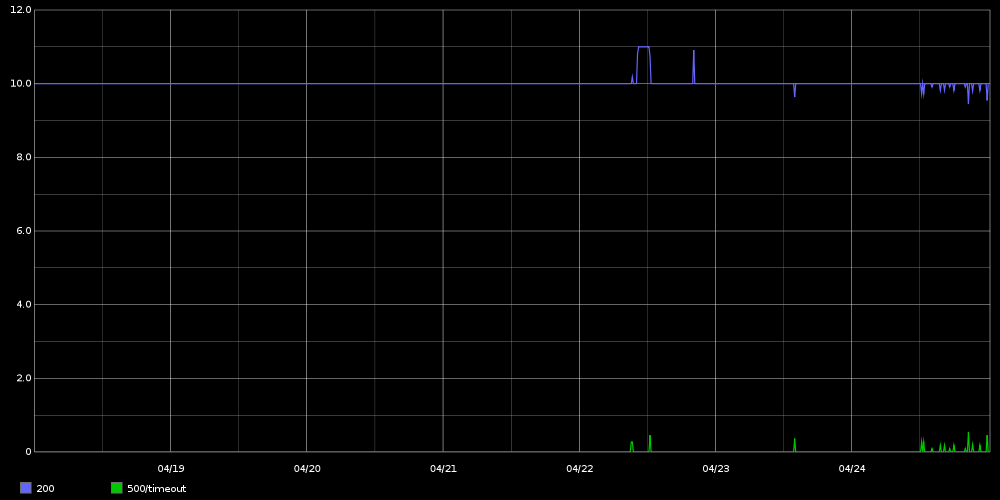
\includegraphics[width=\columnwidth] {images/availability/apr18/authenticator_measurer_small.png}}
  \caption{Heartbeat measurement: Summarized HTTP request status codes for each measurement step for application \emph{authenticator}}
  \label{fig:heartbeat_auth}
\end{figure}

\begin{figure}[ht]
  \fbox{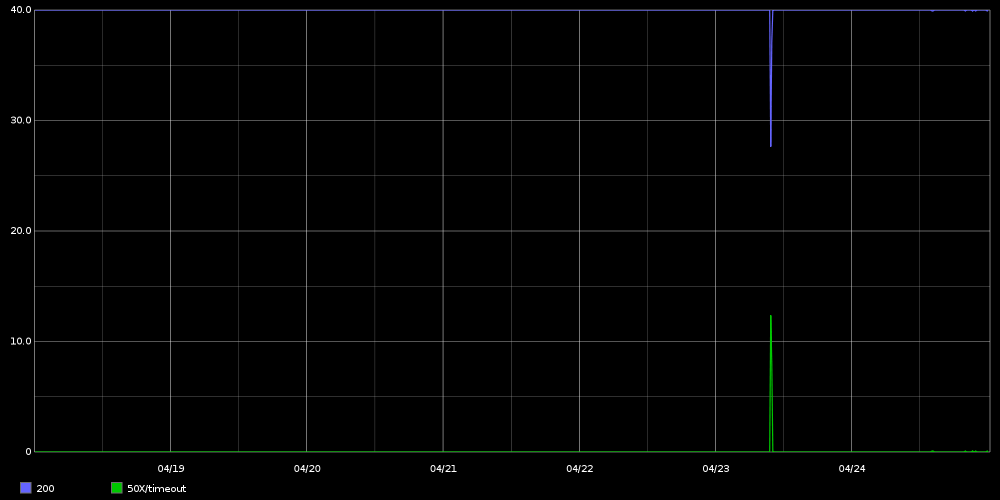
\includegraphics[width=\columnwidth] {images/availability/apr18/threaded_comments_measurer_small.png}}
  \caption{Heartbeat measurement: Summarized HTTP request status codes for each measurement step for application \emph{threaded-comments}}
  \label{fig:heartbeat_tr}
\end{figure}

From the graphs it becomes apparent that when failures occurred, they never affected all instances of a deploy, but only a subset of them. The peak percentages of \emph{down} instances relative to \emph{up} instances are \mytilde6\% for \emph{soundcloud}, \mytilde20\% for \emph{authenticator} and \mytilde57\% for \emph{threaded-comments}. Following this, we define that an application's deploy is \emph{down} in a certain time period, when more than 5\% of all its service instances are \emph{down}.

Table~\ref{tab:heartbeat_failure_probs} shows the results of our measurements as well as the calculated failure probabilities after the equations in \nref{subsec:historical_availability_theory}. As mission time we chose \emph{t = 720 minutes (12hours)}. Using these failure probabilities in the fault tree results in a TOP event probability of \textbf{0,96588}.

\begin{table}[ht]
  \caption{Failure probabilities for application deploys measured via heartbeat measurements from April 18 2014 to April 24 2014 with \emph{down} threshold 5\%. The \emph{mission time} for the failure probability calculation was 720 minutes (12 hours).}
  \label{tab:heartbeat_failure_probs}
  \begin{adjustwidth}{-0.5in}{-.5in}
  \begin{tabular}{ |l|l|l|l|l|l| }
    \hline
    Application & \#Datapoints & \#Up & \#UpSequences & MTTF & Failure probability \\
    \hline
    threaded-comments & 10080 & 10066 & 2 & 5032,50 & 0,1333 \\
    authenticator & 10080 & 10053 & 17 & 591,29 & 0,7040 \\
    soundcloud & 10080 & 9996 & 28 & 356,96 & 0,8669 \\
    \hline
  \end{tabular}
  \end{adjustwidth}
\end{table}

\subsubsection{Discussion}

\emph{Measurer} requested each instance once per time period. We assume that the result of that single request represents the state of the instance for the whole time period. We do not have knowledge about the state of the instance for the rest of the time. Even though this problem could be mitigated by decreasing the measurement interval (for example to one second), it remains a fundamental problem of the method.

For each application we defined one HTTP resource location to query against. Therefore \emph{Measurer} may also only know about the availability of that single resource. Given that an application might show different failure characteristics for different resource locations, the results from our measurement may not capture the complete availability of the instances, as they are experienced by the clients of said instances. Querying more resource locations per instance might mitigate this problem, but its practical applicability is bound to the number of resource locations to query.

During operation the measurements themselves do create load on the instances, thus measuring might alter the results of the measurement. Given that we assume to work with systems that should be able to handle hundreds of requests per second per instance, the effect of measurements should not have a significant impact.
% In our case study execution, this became a problem with the \emph{soundcloud} application, whose service instances handle requests blockingly.

In our investigations we do not guard against network failure. Since we did not experience simultaneous failures of all instances at the same time, we may assume that no total network outage happened during the time of our tests. Still, partial network failures might have altered the results of our measurements.

One of the implicit assumptions we have with this measurement is that our system for executing the measurements experiences no or less failures than the system we measure. This includes \emph{Measurer} as well as \emph{Graphite} (which we used for storing the measurement information). We did not test, as to how much this assumption is true.

Once we had the results from the measurements, we had to decide for each time period if the deploy was \emph{up} or \emph{down}. We based this on a ratio of \emph{up} and \emph{down} instances: if more than 5\% of the instances were \emph{down} we assumed the deploy to be \emph{down}. We set this ratio threshold as a ``good guess'' after manually assessing the collected data. Future work should investigate better ways of assessing the ratio threshold or investigate other ways of making the \emph{up}/\emph{down} assessment for deploys.

\vfill\clearpage

\subsection{Production traffic measurements}
\label{subsec:existing_measurement}

To collect historical availability data of an application deploy, we measured the production traffic for the deploy's service instances. In this section we will explain the method, how we executed it in our case study and discuss our findings.

\subsubsection{Measurement method}

When an application is deployed in the production environment it will serve the production traffic created by the users. Collecting information on that traffic allows us to derive historical availability data.

In our case study we were interested in measuring the three applications \emph{soundcloud}, \emph{authenticator} and \emph{threaded-comments}. All of these have deploys in the production environment. They all use the HTTP~protocol~\cite{rfc2616} to handle requests. For these requests we were able to gather metrics about the returned HTTP status codes from each deploy's service instances. To determine if an application is \emph{up} or \emph{down} for a specific time period we looked at the summed number of requests that returned an HTTP response status code smaller than or equal to \emph{500}. We then set a threshold. If the measured sum was above this threshold we considered the deploy to be \emph{down}.

For measuring the production traffic we used the existing telemetry systems (as outlined earlier in \nref{subsec:telemetry}). Finding the correct telemetry system and metrics within these was a non-trivial task that we executed manually, since it required deep knowledge of the system and measurement architecture. We gathered data for seven days between April 18 2014 and April 24 2014 inclusively.

Next we will explain the exact measurement method for each application deploy and show the respective results:

\paragraph{soundcloud} All traffic to service instances of \emph{soundcloud} goes through \emph{HAProxy}~\cite{haproxy} load balancing servers. The access logs of HAProxy are parsed, aggregated, and saved to \emph{Graphite}. The resolution of the data saved in \emph{Graphite} is 56 minutes. That data is an average of sum per minute over all instances of \emph{HAProxy}. The results can be seen in Figure~\ref{fig:measure_soundcloud}. The \emph{down} threshold was set to 75.

\paragraph{authenticator} Each \emph{authenticator} instance aggregates the HTTP response status codes all requests internally and aggregates them with \emph{Prometheus}. The resolution is 1 minute. The results can be seen in Figure~\ref{fig:measure_auth}. The \emph{down} threshold was set to 20.

\paragraph{threaded-comments} Each \emph{threaded-comments} instance sends the HTTP status code of each response to \emph{statsd}. The resolution is 1 minute. The results can be seen in Figure~\ref{fig:measure_tr}. The \emph{down} threshold was set to 20.

\begin{figure}[ht]
  \fbox{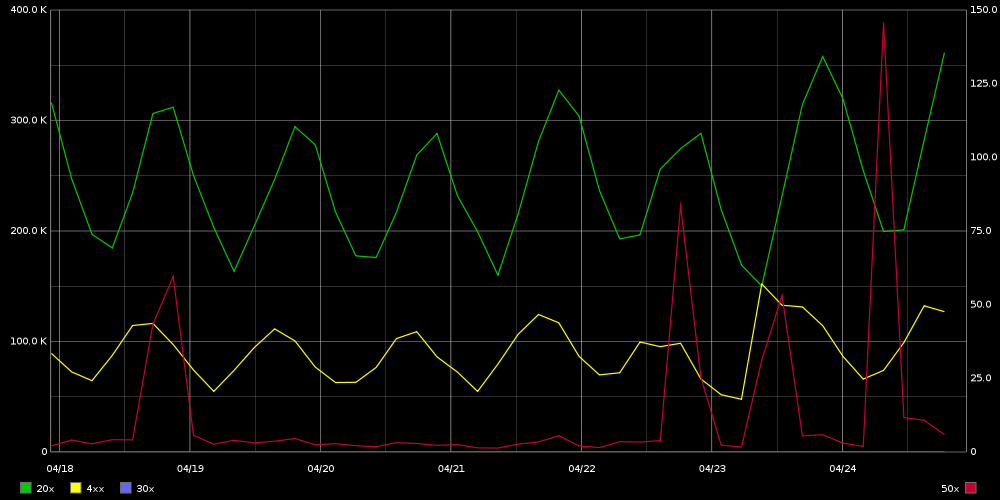
\includegraphics[width=\columnwidth] {images/availability/apr18/soundcloud_haproxy_small.png}}
  \caption{Existing measurements: Summarized HTTP response status codes on \emph{HAProxy} for application \emph{soundcloud}. Please note that there are two y-axes}
  \label{fig:measure_soundcloud}
\end{figure}

\begin{figure}[ht]
  \fbox{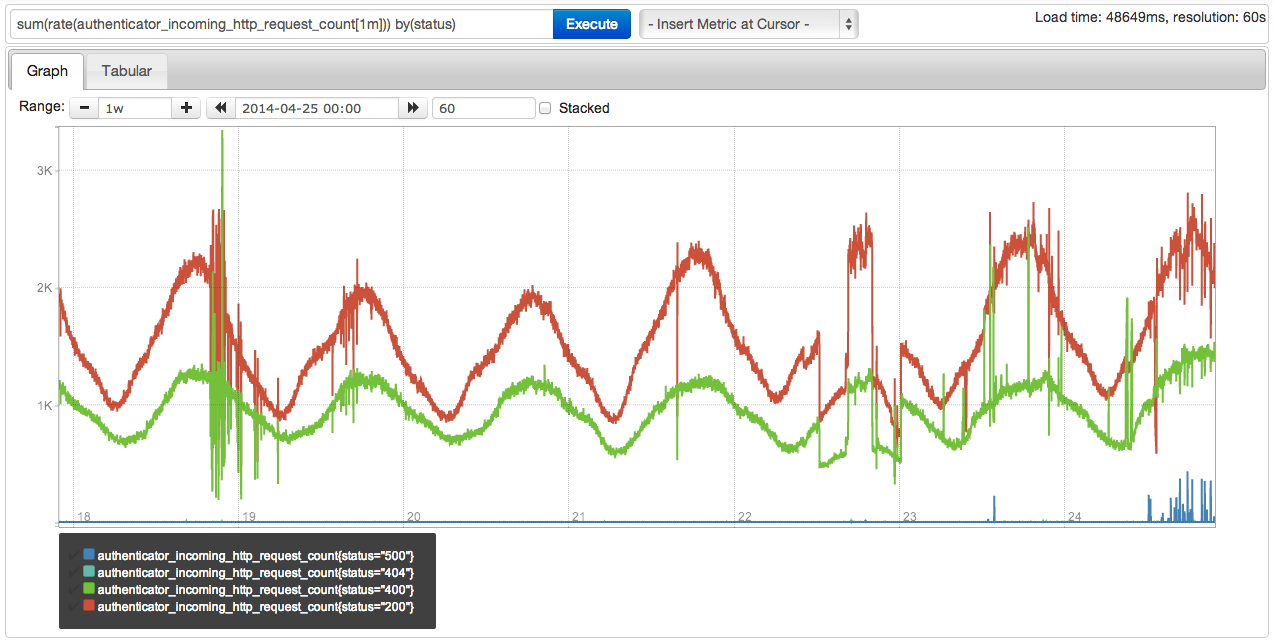
\includegraphics[width=\columnwidth] {images/availability/apr18/authenticator_prometheus_small.png}}
  \caption{Existing measurements: Summarized HTTP response status codes for application \emph{authenticator}}
  \label{fig:measure_auth}
\end{figure}

\begin{figure}[ht]
  \fbox{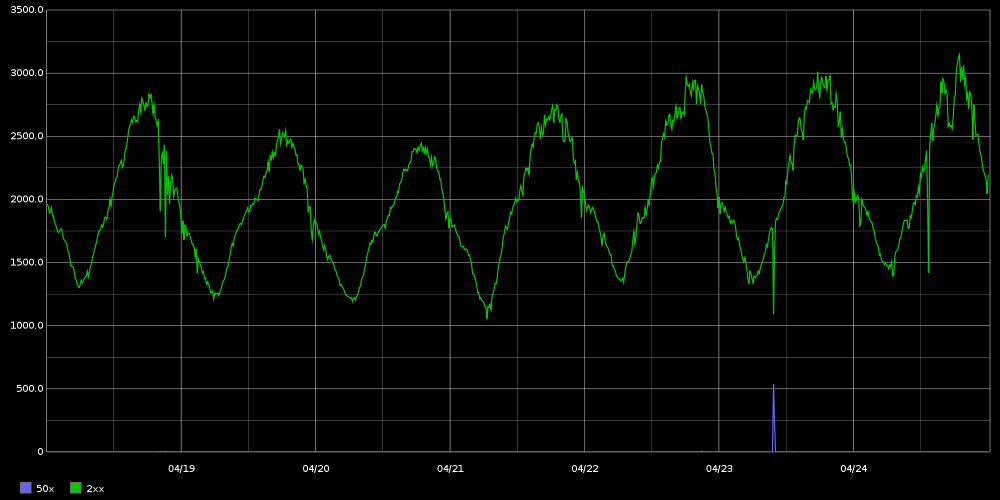
\includegraphics[width=\columnwidth] {images/availability/apr18/threaded_comments_statsd_small.png}}
  \caption{Existing measurements: Summarized HTTP response status codes for application \emph{threaded-comments}}
  \label{fig:measure_tr}
\end{figure}

\subsubsection{Results}

Table~\ref{tab:existing_measure_failure_probs} shows the results of our measurements as well as the calculated failure probabilities after the equations in \nref{subsec:historical_availability_theory}. As mission time we chose \emph{t = 720 minutes (12hours)}. Using these failure probabilities in the fault tree results in a TOP event probability of \textbf{0,96585}.

\begin{table}
  \caption{Failure probabilities for applications measured from production traffic from April 18 2014 to April 24 2014. The \emph{mission time} for the failure probability calculation was 720 minutes (12 hours). Note that we scaled up the datapoints for \emph{soundcloud} to make up for the low granularity provided from the measurement.}
  \label{tab:existing_measure_failure_probs}
  \begin{adjustwidth}{-0.9in}{-.8in}
    \begin{tabular}{ |l|l|l|l|l|l|l|l| }
      \hline
      Application & Threshold & \#Datapoints & \#Ups & \#UpSequences & MTTF & Failure probability \\
      \hline
      soundcloud & 75 & 10080 & 9968 & 3 & 3322,66 & 0,1948 \\
      authenticator & 20 & 10080 & 10037 & 27 & 358,46 & 0,8658 \\
      threaded-comments & 20 & 10080 & 10067 & 2 & 5033,5 & 0,1333 \\
      \hline
    \end{tabular}
  \end{adjustwidth}
\end{table}

\paragraph{Discussion}

In our case study we found two types of how production traffic was measured: \emph{Threaded-comments} and \emph{authenticator} are measured internally, within the instance processes. \emph{Soundcloud} is measured externally, on the load balancer between service consumers and service instances. Both measure the actual service consumer traffic. We believe the external measurements to be more accurate: If a service instance crashes the internal measurement will equally crash and therefore not count failed requests anymore. External measurements can count instance crashes without problems. The assumption with external measurements is then that the complete production traffic is measured on that measuring point. For example in our case study the external measurements happened on the load balancers. We verified that the service instances were not serving production traffic routed through other means. If that would be the case, the other means would have to be incorporated into the external measurements as well.

In our case study the time period resolution of the measurements varied with 56 minutes for \emph{soundcloud} and 1 minute for \emph{threaded-comments} and \emph{authenticator}. This led to an exaggeration of the downtime that we measured for \emph{soundcloud}, which we scaled up to match the resolution of the other measurements. We believe that a high resolution (preferably in the seconds not minutes range) as well as the same resolution for all measurements would improve the quality of the results.

Once we had the results from the measurements, we had to decide for each time period if the deploy was \emph{up} or \emph{down}. We based this on a threshold value of failed responses based on the delivered HTTP status code. We set this threshold as a ``good guess'' after manually assessing the collected data. Future work should investigate better ways of assessing the threshold or investigate other ways of making the \emph{up}/\emph{down}.

\subsection{Discussion}
\label{subsubsec:measure_discussion}

Both approaches measure the perspective of the service consumers and how these experience the service. We believe this to be a good perspective for measuring historical availability since failures are the entity that impedes on a service's availability and failures may only be experienced (and therefore measured) from the service consumer's perspective.

We believe that the \emph{production traffic} approach will deliver more accurate data. We base this opinion on two arguments: The \emph{heartbeat} measurement may only measure a limited number of HTTP resources, whereas the \emph{production traffic} approach will measure all relevant resources, given that these are used by the actual service consumers. Secondly the \emph{heartbeat} approach has the problem of choosing appropriate querying intervals. In the \emph{production traffic} approach, this problem does not exist since the querying intervals are implicitly chosen by the service consumer traffic. If we assume that a service instance serves several hundred requests per second, the effective querying interval in the \emph{production traffic} approach is in the range of milliseconds.

For both approaches we split time into a time series with equal time periods. In both approaches we then had the problem of deciding for each time period, if a deploy as \emph{up} or \emph{down} for that period. In both cases we based this decision on a threshold which we set as a ``good guess''. Depending on the measured data and the chosen threshold value, the resulting \emph{up}/\emph{down} periods may look significantly different. We believe this to be a crucial problem of the methods. Future work should investigate this aspect more.

Next we will compare the resulting MTTFs of both methods in  \autoref{tab:heartbeat_failure_probs} and \autoref{tab:existing_measure_failure_probs}. The MTTFs of \emph{threaded-comments} are nearly the same (\emph{heartbeat}: 5032,50 and \emph{production traffic} 5033,5). The MTTF of the \emph{authenticator} \emph{heartbeat} measurement (591,29) is \mytilde65\% higher than the \emph{production traffic} measurement (358,46). The MTTF of the \emph{soundcloud} \emph{heartbeat measurement} (356,96) is \mytilde10\% of the \emph{production traffic} measurement (3322,66). The lowest MTTFs of both methods are nearly the same (358,46 and 356,96).

\subsubsection{TOP event probability calculation}

Given that we have the historical availability time series for each of the application deploys we need to calculate the failure probability for of them.

First we calculate the MTTF and with that the failure rate. Basis for this calculation is the assumption that the system has reached steady-state. Thus given that our observation period was one week, we assume that all other weeks yield similar MTTF values than the one we observed. This is a weak assumption, since we know from experience that the availability of deploys may differ significantly between weeks. One aspect to investigate for mitigating this effect is observing over longer periods of time.

Based on the failure rate, we may calculate the failure probability. For this we have to assume a failure distribution. We chose the exponential distribution (\autoref{eq:failureprob}) since it allows for analytical calculation. Future work should investigate to which extent it represents failures of application deploys well and if other distributions might be better suited. The exponential distribution equation needs a mission time for calculating the failure probability. We chose 720 minutes as a mission time as a ``good guess''. Intuitively, the higher the mission time, the higher the resulting failure probabilities will be.

Given the failure probabilities for the basic events, we may calculate the TOP event probability of the fault tree. When comparing the two results (\emph{heartbeat approach}: \emph{0,96588} and \emph{production traffic approach}: \emph{0,96585}) we can see that they are very similar, despite the fact that the MTTFs of the individual applications do differ significantly. We attribute the similarity to the fact that the basic event with the highest failure probability has the most significant impact on the calculated TOP event probability. Given that we have seen that the lowest MTTFs of both case study executions is nearly the same, the highest failure probabilities are equally similar, thus leading to similar TOP event probabilities.

One of the assumption when using fault tree basic event probabilities is that they are stochastically independent. When measuring historical availability, this assumption is not necessarily fulfilled, given that applications do depend on each other. We did not investigate this aspect during our measurements. We see opportunity in future work differentiating between ``inherent'' failure and ``propagated'' failure of an application.

\section{Discussion}
\label{sec:quant_discussion}

In this section we will discuss the findings from this chapter, compare the methods we investigated and hint to potential for future work.

In this chapter we have investigated options for creating a quantified fault tree. We based these investigations on the qualitative fault tree constructed in earlier \nref{chapter:fault_trees}. Given such a qualitative fault tree, we may assign failure probabilities to the basic events of the fault tree in order to calculate the TOP event probability. For the fault tree we used in our case study execution, we have shown the equation at the beginning of this chapter in \autoref{eq:quant_prob}.

For obtaining basic event failure probabilities, we investigated four methods: two methods based on \emph{source code metrics} (\nref{sec:source_code}) and two methods based on \emph{historical availability} of application deploys (\nref{sec:historical_availability}). The focus of this work was to investigate the feasibility of the approaches in the context of our case study. We found all approaches to be executable. We did not gather enough information to do a meaningful quantitative analysis, but rather see our work as proof that it is possible to do such analyses.

Comparing the four approaches regarding the numerical values of the TOP event probability is not a fruitful task, since all methods at some point in their execution rely on a threshold or normalization chosen by the user. Still it is possible to qualitatively compare them, which we will do next.

\subsubsection{Mapping application identifiers}

For the methods based on \emph{source code metrics} it was easy to map application identifiers to the respective codebase and source code management repository, since as assumption we earlier established in \nref{sec:software_environment_terminology} that all applications have exactly one codebase with canonical repository location. For \emph{historical availability} this process was a bigger problem. In practice, \emph{historical availability} may only be measured from concrete service instances. The measured values may then be aggregated to represent the deploy, which in turn may be taken as the representation of the application. We were interested in the perspective of applications and dependencies between them since we took that perspective in earlier investigations \nref{chapter:dependency_graph} and \nref{chapter:fault_trees} as well. An opportunity for future work is to use an approach based on service instances. Building the dependency graph and qualitative fault tree might then contribute from our experiences of measuring network traffic as introduced in \nref{subsec:from_network}.

\subsubsection{External applications}

\emph{Lines of code} was the only method with which we calculated probabilities for external applications. We assumed \emph{relative code churn} to not be expressive for external applications, since during our investigations no new versions of the external applications were deployed in our case study. With \emph{historical availability} measurement, we found no representative existing \emph{production traffic measurement} and therefore also did not investigate \emph{external heartbeat measurements} further. Even though we did not execute these methods for external applications in our case study, technically these should be well feasible.

\subsubsection{Source code metrics}

When we executed the \emph{lines of code} method in our case study, it revealed big differences in the size of codebases. Given that we linearly normalized the lines of code to failure probabilities, this led to the over-emphasis of large codebases and the neglectable impact of smaller ones. Future work may investigate, how different mapping functions from \emph{lines of code} to failure probabilities might impact the results.

The calculated \emph{relative code churn} numbers from our case study fluctuated between 0 and \mytilde0,6 depending on the chosen time periods. Also a property of \emph{relative code churn} is that it cumulatively increases with increasing time periods. Fluctuation and cumulation make comparing relative code churn numbers and resulting failure probabilities hard to compare with other methods. Given the assumption that it is a good predictor of failure probabilities, we believe it may be used as an indicator for potential dependability risks. For example application developers could be notified when their service dependency applications show an increase in failure probability based on \emph{relative code churn}.

In our work we only investigated two approaches based on \emph{source code metrics}. Many more exist, which may be investigated in future work. The work by D'Ambros et al \cite{DAmbros2011} surveying defect prediction approaches may provide a good starting point.

\subsubsection{Historical availability}

During our investigation in the case study we found both methods for measuring \emph{historical availability} feasible. We believe that \emph{production traffic measurements} are to be preferred over \emph{heartbeat measurements}, since they test more resources and do not have the problem of choosing an appropriate test interval. We furthermore believe that they are well integrateable in existing measurement systems, thus lowering the complexity for implementation.

One potential problem we noticed, but did not investigate thoroughly, is the difference between ``internal'' and ``propagated'' failures of a service instance. Given that we see that a service instance is unavailable, we do not know if the failure is from within the application itself (``internal'') or cause by another application failing (``propagated''). An opportunity to investigate this in future work is to correlate failures over time, over several systems as well from the users' perspective. We tried to do this in our case study, but during our investigation periods no problems surfaced that allowed for meaningful correlation. In our investigations we therefore assumed all noticed failures to be of ``internal'' nature.

Another interesting opportunity for future work is the decomposition of services into separate resources or functionalities. Each may then be measured individually for its availability. This would allow for more fine-grained fault trees and failure correlations, which would allow more detailed insights into the architecture.

\subsubsection{Reliability for repairable systems}

In the way we used fault trees here, the TOP event probability denotes the unreliability of the investigated system, without taking repairs into consideration. We believe software always to be repairable (most fundamentally by restarting it). Future work might investigate how to reflect this property in fault tree investigation.

\subsubsection{Duplicated basic events}

In the fault tree we used (\autoref{fig:fault_tree_threaded_comments}) there are no duplicate basic events. Our method for calculating the TOP event probability requires all basic event to be stochastically independent. This can be a problem, since there is no guarantee that in the methods we introduced. In practice, once two separate applications (\emph{A} and \emph{B}) depend on the same other application (\emph{C}), then that application \emph{C} will be represented twice in the resulting fault tree. Examples can be seen in \autoref{fig:fault_tree_v2}, where the basic event ``5'' exists many times.

\subsubsection{Investigate change}

Our investigations with \emph{code churn} are the only ones that allow for looking at changes of the resulting TOP event probability over time. We see potential in further investigating this with the other methods, especially how changes to an application do impact the TOP event probability. Looking at changes over time would also allow for comparing the results of the methods better, since it would be possible to correlate changes.

\section{Summary}

In this chapter we investigated approaches to constructing a quantitative fault tree. Given a qualitative fault tree the TOP event probability may be calculated if basic event probabilities exist. We investigated two types of methods for gathering basic event probabilities for applications: source code metrics and historical availability. The two source code metrics \emph{lines of code} and \emph{relative code churn} are known to allow prediction of defects. We proposed to extend these metrics for calculating failure probabilities. Similarly, \emph{historical availability measurements} allow the calculation basic event probabilities. We proved the feasibility of these methods by executing them in our case study and gathered promising results, but more work is needed to quantifiably evaluate these.